\documentclass[11pt]{article}

\usepackage{amsmath,amssymb}
\usepackage{amsthm}
\usepackage{graphicx}
\usepackage{booktabs}
\usepackage{hyperref}
\usepackage{geometry}
\usepackage{algorithm}
\usepackage{algpseudocode}
\usepackage{caption}
\usepackage{subcaption}
\usepackage{tikz}
\usepackage{pgfplots}
\usepackage{pgfplotstable}
\usepackage{placeins}
\usepackage{float}
\pgfplotsset{compat=1.18}

% Path to benchmark data (different for article vs SEA version)
\newcommand{\rootdir}{.}

% Load benchmark metadata from CSV
\pgfplotstableread[col sep=comma]{\rootdir/figures/rust/metadata.csv}\rustmetadata
\pgfplotstablegetelem{0}{value}\of\rustmetadata \let\rustbenchmarkdate\pgfplotsretval
\pgfplotstablegetelem{1}{value}\of\rustmetadata \let\rustbenchmarkmachine\pgfplotsretval
\pgfplotstablegetelem{2}{value}\of\rustmetadata \let\rustbenchmarkn\pgfplotsretval
\pgfplotstablegetelem{3}{value}\of\rustmetadata \let\rustbenchmarkiterations\pgfplotsretval

% Command to add benchmark note to figures
\newcommand{\rustbenchmarknote}{\par\vspace{2pt}\noindent{\scriptsize\textit{Benchmarked on \rustbenchmarkmachine\ (\rustbenchmarkdate), $n=\rustbenchmarkn$, \rustbenchmarkiterations\ iterations.}}}
\usetikzlibrary{positioning,arrows.meta,patterns,calc,decorations.pathreplacing,pgfplots.fillbetween}

\geometry{margin=1in}

% Theorem environments
\newtheorem{theorem}{Theorem}
\newtheorem{lemma}[theorem]{Lemma}
\newtheorem{corollary}[theorem]{Corollary}
\newtheorem{proposition}[theorem]{Proposition}
\theoremstyle{definition}
\newtheorem{definition}[theorem]{Definition}
\newtheorem{example}[theorem]{Example}
\theoremstyle{remark}
\newtheorem{remark}[theorem]{Remark}
\newtheorem{claim}[theorem]{Claim}

\title{DeltaSort: Incremental repair of sorted arrays with known updates}
\author{Shubham Dwivedi \\
\small Independent Researcher \\
\small \texttt{shubd3@gmail.com}
}
\date{2026}

\begin{document}
\maketitle

\begin{abstract}
Reading sorted values or records is a fundamental operation in many systems. When records need to be read in a particular order, sorting-on-read incurs repeated $O(n \log n)$ cost which can become a bottleneck in read-heavy systems. A standard solution is to have a derived sorted read-replica that is updated with the latest snapshot asynchronously whenever the system-of-record gets updated. For updating read-replicas, existing approaches rely on either full re-sorting or incremental techniques such as Binary-Insertion-Sort or Extract–Sort–Merge. In this paper, we show how to do better than these approaches for certain update batch sizes. First, we formulate an alternative model in which the sorting routine is explicitly informed of the updated indices since the previous sort. Under this model, we present \emph{DeltaSort}, an efficient incremental repair algorithm for arrays. We present theoretical analysis and experimental evidence that show that \emph{DeltaSort} outperforms existing approaches for a range of update batch sizes. These results suggest that tighter integration between update pipelines and sorting routines can yield significant performance gains in practice. We also explore limitations of this approach and identify a crossover point, depending on array size, where full re-sorting becomes preferable over \emph{DeltaSort}. 
\end{abstract}

%==============================================================================
\section{Introduction}
%==============================================================================

Sorting is among the most optimized primitives in modern systems, backed by decades of deep research. Standard library implementations---TimSort~\cite{timsort}, Introsort~\cite{musser1997introspective}, and PDQSort~\cite{peters2021pdqsort} deliver excellent performance for general inputs by exploiting partial order, cache locality, and adaptive strategies. However, these algorithms operate under a \emph{blind} model: they discover structure dynamically rather than being explicitly informed about which values have changed since the previous sort.

In many practical systems, this assumption is unnecessarily pessimistic. Sorted arrays are often maintained incrementally in read-heavy workloads where updates affect only a subset of values and the indices of those updates can be easily tracked if needed. Nevertheless, this information is typically not tracked or utilized, and systems fall back to blind re-sorting or standard repair approaches using Binary-Insertion-Sort or Extract-Sort-Merge, depending on the update batch size.

As an example, consider a web application that shows a real-time game leaderboard sorted by score. Being able to efficiently update the sorted view on updates directly impacts the user experience. 

Consider an analytics service that supports queries over telemetry records sorted by a particular field. The underlying data is distributed across multiple clusters, and query results are materialized and cached to serve repeated reads efficiently. As the base data sources receive updates, the cached sorted result must either be invalidated and recomputed, or incrementally updated to reflect the changes. Cache invalidation is the simplest approach, but it forces a full re-fetch and re-sort of the result even when updates are sparse. An alternative is to incrementally repair the cached sorted array as updates arrive from the underlying sources. In this setting, updates are naturally identified by key, and their positions in the cached result are known or can be tracked. Applying incremental sorting techniques such as DeltaSort allows the cached result to be updated in place, avoiding repeated full re-sorts. At scale—where many users issue similar queries and updates arrive continuously—this distinction can have a significant impact on both latency and resource utilization. Incremental repair enables systems to trade occasional localized reordering for improved steady-state performance under read-heavy workloads.

The traditional approaches aren't optimal have limitations: Full re-sorting is expensive for small updates, Binary-Insertion-Sort incurs high write cost ($O(kn)$) for large update batches, and Extract-Sort-Merge uses $O(n)$ auxiliary space even for small updates. To address these limitations, this paper makes the following contributions:

\begin{enumerate}
  \item \textbf{Update-aware sorting model:}
  We formulate a sorting model in which the sorting routine is explicitly informed of the updated indices since the previous sort. Under this model, Binary-Insertion-Sort and Extract-Sort-Merge serve as the baseline algorithms because they already assume knowledge of what has been updated. Table~\ref{tab:incremental-sorting-algorithms} summarizes the key characteristics of these algorithms under the update-aware model.

  \item \textbf{DeltaSort algorithm:}
  We present \emph{DeltaSort}, an incremental repair algorithm for sorted arrays designed for the update-aware model. DeltaSort batches multiple updates and achieves multi-fold speedups over traditional approaches for a wide range of update batch sizes.

  \begin{table}
\centering
\caption{Algorithms for update-aware sorting}
\label{tab:incremental-sorting-algorithms}
\begin{tabular}{l c c}
\toprule
Algorithm & Time (Expected / Worst) & Space \\
\midrule
Binary-Insertion-Sort$^{\dagger}$ & $O(kn)$ & $O(1)$ \\
Extract–Sort–Merge$^{*}$$^{\dagger}$ & $O(k \log k + n)$ & $O(n)$ \\
\textbf{DeltaSort}$^{*}$ & $O(n\sqrt{k})\,/\,O(kn)$ & $O(k)$ \\
\bottomrule
\end{tabular}

\vspace{0.3em}
{$n$ = array size, $k$ = number of updates}

\small $^{*}$These use a full sort primitive internally assumed to run in $O(k \log k)$ time and $\le O(k)$ space.

\small $^{\dagger}$These have the same expected and worst case time complexity.
\end{table}

\end{enumerate}

%==============================================================================
\section{Related Work}
\label{sec:related}
%==============================================================================

%TODO: Talk about parallelizable sorting algorithms

Adaptive sorting algorithms exploit existing order in the input to improve performance on nearly sorted data. TimSort~\cite{timsort} and natural merge sort~\cite{knuth1998art} dynamically identify monotonic runs and merge them efficiently, while a substantial body of work formalizes measures of presortedness and analyzes sorting complexity as a function of these measures rather than input size alone~\cite{mannila1985measures}. These approaches, however, operate under a blind model: partial order must be rediscovered through full-array scans, and no external information about which values have changed is assumed.

A separate line of work studies incremental computation and view maintenance in database and streaming systems, where changes to input data are propagated to derived results using explicit delta representations~\cite{gupta1995maintenance, nikolic2014incremental, akidau2015dataflow}. These techniques focus on maintaining query results, aggregates, and materialized views, and operate at the level of relational or dataflow operators rather than array-based sorting primitives. While they demonstrate the practical value of update-aware computation, they do not specifically address the problem of efficiently restoring sorted order in arrays under batched point updates.

Dynamic data structures offer a different trade-off. Self-balancing trees such as AVL trees~\cite{avl1962}, red--black trees~\cite{guibas1978dichromatic}, B-trees~\cite{bayer1972organization}, and skip lists~\cite{pugh1990skip} support efficient ordered updates with logarithmic cost, but abandon contiguous array layout and its associated advantages.

In contrast, this work considers maintaining sorted order in arrays where the indices of updated values since the previous sort are explicitly available. Unlike adaptive sorting algorithms, which need to discover the presortedness, \emph{DeltaSort} already knows which values have changed and hence can leverage this information to achieve better performance. Unlike incremental view maintenance techniques, which focus on higher-level query results, \emph{DeltaSort} is a low-level sorting primitive for arrays which can be used by higher level systems. Unlike dynamic data structures, which sacrifice array layout for update efficiency, \emph{DeltaSort} maintains the contiguous array layout.

%==============================================================================
\section{Problem Model}
\label{sec:model}
%==============================================================================

\begin{definition}[Update-Aware Sorting]
\label{def:problem}
Let $A[0..n-1]$ be an array sorted according to a strict weak ordering defined by a comparator $\texttt{cmp}$. Let $U = \langle u_0, u_1, \dots, u_{k-1} \rangle$ be a sequence of indices such that \[ 0 \le u_0 < u_1 < \dots < u_{k-1} \le n-1, \] and the values at these indices may have been arbitrarily updated, while values at all other indices remain unchanged. The \emph{update-aware sorting problem} is to restore $A$ to a state that is sorted with respect to $\texttt{cmp}$, given explicit knowledge of the set $U$.
\end{definition}

\begin{remark}
The above model can be easily extended to account for additions and deletions from the array-
\begin{itemize}
  \item \textbf{Addition:} For an existing array of size $n$, append new value to end of the array and add $n$ (the new index) to $U$. 
  \item \textbf{Deletion:} To delete value at index $i$, set its value to a sentinel $\infty$ that is greater than all other values according to $\texttt{cmp}$ and add it to $U$. Once sorted, the array size can be reduced by one removing the last element.
\end{itemize}
\end{remark}

%==============================================================================
\section{DeltaSort Algorithm}
\label{sec:algorithm}
%==============================================================================

\subsection{Overview}

Before we get to how the algorithm works, let's establish useful terminology-

\begin{definition}[Direction]
\label{def:direction}
For an updated index $i$, we define its \emph{direction} based on local order:
\begin{itemize}
  \item \textbf{LEFT ($L$)}: Value \textbf{must} move left---$\texttt{cmp}(A[i-1], A[i]) > 0$ (for $i > 0$).
  \item \textbf{RIGHT ($R$)}: Value \textbf{may} move right and \textbf{cannot} move left.
\end{itemize}
\end{definition}

\begin{remark}
The definition of direction is deliberately asymmetric: L requires a definite violation ($A[i-1] > A[i]$), while R encompasses both violations and non-violations. One might consider a three-way classification with a separate STABLE direction for values already in their correct position. However, this complicates the algorithm:
\begin{enumerate}
  \item STABLE values would be processed identically to R values (both may stay or move right).
  \item Fixing an R value can shift elements, potentially converting a previously STABLE neighbor into an R violation.
\end{enumerate}
The two-way classification avoids this issue by maintaining a useful invariant: \emph{the direction of an updated index never changes during Phase~2}. An L stays L until fixed; an R stays R until fixed. This simplifies both the correctness argument and implementation.
\end{remark}

\begin{definition}[Segment]
\label{def:segment}
A \emph{segment} is a pair of indices $(i, j)$ with $i < j$ satisfying:
\begin{enumerate}
  \item Either $i = 0$, or $i \in U$ with direction R.
  \item Either $j = n - 1$, or $j \in U$ with direction L.
  \item There do not exist updated indices $p, q \in U$ with $i < p < q < j$ such that $p$ has direction L and $q$ has direction R.
\end{enumerate}
Intuitively, a segment is a contiguous portion of the array where all R-direction updates precede all L-direction updates. Condition~(3) ensures that no L appears before an R within the segment. Conditions~(1) and~(2) handle boundary cases: a leading segment containing only L's is bounded by the array start, and a trailing segment containing only R's is bounded by the array end. Figure~\ref{fig:segment-structure} illustrates this structure.
\end{definition}

% Figure: Segment structure diagram
\begin{figure}[H]
\centering
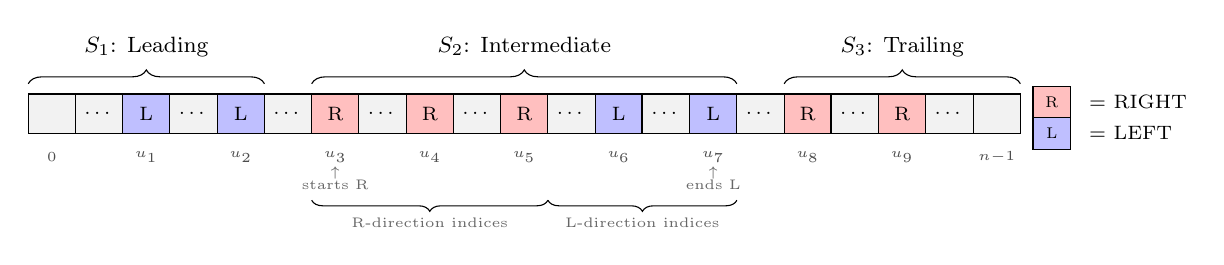
\begin{tikzpicture}[
    cell/.style={minimum width=0.6cm, minimum height=0.5cm, draw, font=\scriptsize},
    dotcell/.style={minimum width=0.5cm, minimum height=0.5cm, font=\scriptsize},
    indexcell/.style={minimum width=0.6cm, font=\tiny, text=black!70},
    right/.style={cell, fill=red!25},
    left/.style={cell, fill=blue!25},
    clean/.style={cell, fill=gray!10, font=\scriptsize},
    segbrace/.style={decorate, decoration={brace, amplitude=5pt}},
    segbracem/.style={decorate, decoration={brace, amplitude=4pt, mirror}},
    seglabel/.style={font=\footnotesize},
    condlabel/.style={font=\tiny, text=black!60},
    faded/.style={opacity=0.4}
]

% Array indices (shown below)
\def\yidx{-0.55}
\def\yarr{0}

% === ARRAY START ===
\node[clean] at (-0.9, \yarr) {};
\node[indexcell] at (-0.9, \yidx) {$0$};
\node[clean] at (-0.3, \yarr) {\dots};

% === LEADING SEGMENT (L's only, bounded by array start) ===
\node[left] (l0) at (0.3, \yarr) {L};
\node[indexcell] at (0.3, \yidx) {$u_1$};
\node[clean] at (0.9, \yarr) {\dots};
\node[left] (l1) at (1.5, \yarr) {L};
\node[indexcell] at (1.5, \yidx) {$u_2$};

% Inter-segment clean region
\node[clean] at (2.1, \yarr) {\dots};

% === MIDDLE SEGMENT (R's then L's) ===
\node[right] (r1) at (2.7, \yarr) {R};
\node[indexcell] at (2.7, \yidx) {$u_3$};
\node[clean] at (3.3, \yarr) {\dots};
\node[right] (r2) at (3.9, \yarr) {R};
\node[indexcell] at (3.9, \yidx) {$u_4$};
\node[clean] at (4.5, \yarr) {\dots};
\node[right] (r3) at (5.1, \yarr) {R};
\node[indexcell] at (5.1, \yidx) {$u_5$};
\node[clean] at (5.7, \yarr) {\dots};
\node[left] (l2) at (6.3, \yarr) {L};
\node[indexcell] at (6.3, \yidx) {$u_6$};
\node[clean] at (6.9, \yarr) {\dots};
\node[left] (l3) at (7.5, \yarr) {L};
\node[indexcell] at (7.5, \yidx) {$u_7$};

% Inter-segment clean region
\node[clean] at (8.1, \yarr) {\dots};

% === TRAILING SEGMENT (R's only, bounded by array end) ===
\node[right] (r4) at (8.7, \yarr) {R};
\node[indexcell] at (8.7, \yidx) {$u_8$};
\node[clean] at (9.3, \yarr) {\dots};
\node[right] (r5) at (9.9, \yarr) {R};
\node[indexcell] at (9.9, \yidx) {$u_9$};

% === ARRAY END ===
\node[clean] at (10.5, \yarr) {\dots};
\node[clean] at (11.1, \yarr) {};
\node[indexcell] at (11.1, \yidx) {$n{-}1$};

% === SEGMENT BRACES (top) ===
% Leading segment
\draw[segbrace] (-1.2, 0.38) -- (1.8, 0.38);
\node[seglabel] at (0.3, 0.85) {$S_1$: Leading};

% Middle segment
\draw[segbrace] (2.4, 0.38) -- (7.8, 0.38);
\node[seglabel] at (5.1, 0.85) {$S_2$: Intermediate};

% Trailing segment
\draw[segbrace] (8.4, 0.38) -- (11.4, 0.38);
\node[seglabel] at (9.9, 0.85) {$S_3$: Trailing};

% === SUB-BRACES for middle segment (bottom) ===
\draw[segbracem] (2.4, -1.1) -- (5.4, -1.1);
\node[condlabel, anchor=north] at (3.9, -1.2) {R-direction indices};
\draw[segbracem] (5.4, -1.1) -- (7.8, -1.1);
\node[condlabel, anchor=north] at (6.6, -1.2) {L-direction indices};

% === ANNOTATIONS for boundary conditions ===
% Condition markers (centered on cells)
\node[condlabel] at (2.7, -0.75) {$\uparrow$};
\node[condlabel] at (2.7, -0.9) {starts R};

\node[condlabel] at (7.5, -0.75) {$\uparrow$};
\node[condlabel] at (7.5, -0.9) {ends L};

% === LEGEND ===
\node[right, scale=0.8] at (11.8, 0.15) {R};
\node[font=\scriptsize, anchor=west] at (12.15, 0.15) {= RIGHT};
\node[left, scale=0.8] at (11.8, -0.25) {L};
\node[font=\scriptsize, anchor=west] at (12.15, -0.25) {= LEFT};

\end{tikzpicture}
\caption{A segment $(i,j)$ starts at either index $0$ or an R-direction updated index, and ends at either index $n{-}1$ or an L-direction updated index, with all R's preceding all L's within. In this example, the leading segment $S_1$ contains only L's (starting from index $0$), the intermediate segment $S_2$ contains R's followed by L's, and the trailing segment $S_3$ contains only R's (ending at index $n{-}1$). Leading and trailing segments may or may not be present depending on the directions of updated indices.}
\label{fig:segment-structure}
\end{figure}

Armed with these definitions, we can see how DeltaSort works. It operates in two phases:

\begin{enumerate}
  \item \textbf{Phase 1 (Segment):} Extract updated values, sort them, and write back to updated indices in index order. This establishes segments (Definition~\ref{def:segment}) in the array that are disjoint and can be \emph{repaired independently}.
  \item \textbf{Phase 2 (Repair):} Repair each segment left-to-right, deferring R indices to a stack until the first L index is encountered. When a L is encountered, first flush and repair all pending Rs in LIFO order, then repair the L. Continue left-to-right.
\end{enumerate}

Figure~\ref{fig:delta-sort-example} illustrates the full DeltaSort process on a small example.

% Example figure showing segmentation with concrete array
\begin{figure}[t]
\centering
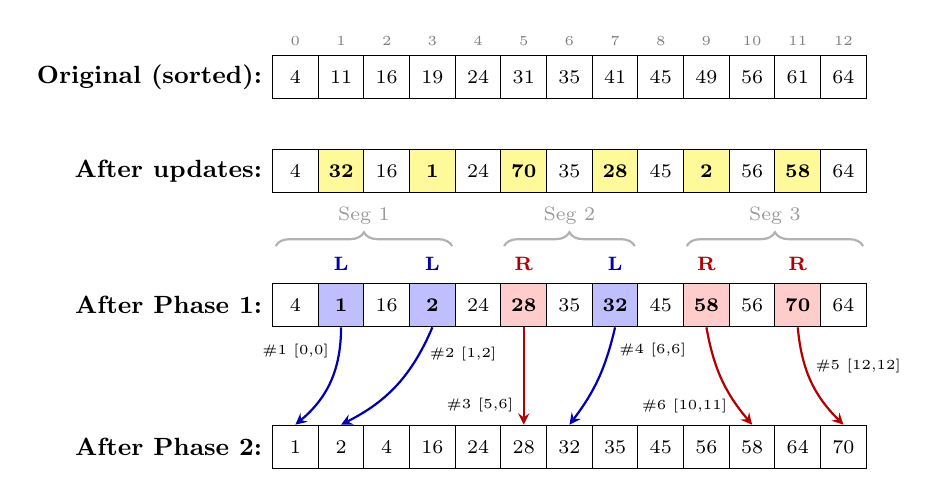
\begin{tikzpicture}[
    cell/.style={draw, minimum width=0.58cm, minimum height=0.55cm, font=\scriptsize},
    cellup/.style={cell, fill=yellow!40, font=\scriptsize\bfseries},
    cellL/.style={cell, fill=blue!25, font=\scriptsize\bfseries},
    cellR/.style={cell, fill=red!20, font=\scriptsize\bfseries},
    larrow/.style={->, >=stealth, thick, blue!70!black},
    rarrow/.style={->, >=stealth, thick, red!70!black},
    segbrace/.style={decorate, decoration={brace, amplitude=5pt}},
]

% === STAGE 1: Original sorted array ===
\node[font=\small\bfseries, anchor=east] at (-0.3, 0) {Original (sorted):};
\foreach \i/\v in {0/4, 1/11, 2/16, 3/19, 4/24, 5/31, 6/35, 7/41, 8/45, 9/49, 10/56, 11/61, 12/64} {
    \node[cell] (o\i) at (\i*0.58, 0) {\v};
}
% Index labels
\foreach \i in {0,...,12} {
    \node[font=\tiny, gray] at (\i*0.58, 0.45) {\i};
}

% === STAGE 2: After updates applied ===
\node[font=\small\bfseries, anchor=east] at (-0.3, -1.2) {After updates:};
\foreach \i/\v/\up in {0/4/0, 1/32/1, 2/16/0, 3/1/1, 4/24/0, 5/70/1, 6/35/0, 7/28/1, 8/45/0, 9/2/1, 10/56/0, 11/58/1, 12/64/0} {
    \ifnum\up=1
        \node[cellup] (u\i) at (\i*0.58, -1.2) {\v};
    \else
        \node[cell] (u\i) at (\i*0.58, -1.2) {\v};
    \fi
}

% === STAGE 3: After Phase 1 (sorted updates, L/R classified) ===
\node[font=\small\bfseries, anchor=east] at (-0.3, -2.9) {After Phase 1:};

% Segment braces (between Stage 2 and L/R labels)
\draw[segbrace, thick, gray!60] (0*0.58-0.25, -2.15) -- (3*0.58+0.25, -2.15) 
    node[midway, above=4pt, font=\scriptsize, gray!80] {Seg 1};
\draw[segbrace, thick, gray!60] (5*0.58-0.25, -2.15) -- (7*0.58+0.25, -2.15) 
    node[midway, above=4pt, font=\scriptsize, gray!80] {Seg 2};
\draw[segbrace, thick, gray!60] (9*0.58-0.25, -2.15) -- (12*0.58+0.25, -2.15) 
    node[midway, above=4pt, font=\scriptsize, gray!80] {Seg 3};

% L/R labels (just above Phase 1 array)
\node[font=\scriptsize, blue!70!black] at (1*0.58, -2.38) {\textbf{L}};
\node[font=\scriptsize, blue!70!black] at (3*0.58, -2.38) {\textbf{L}};
\node[font=\scriptsize, red!70!black] at (5*0.58, -2.38) {\textbf{R}};
\node[font=\scriptsize, blue!70!black] at (7*0.58, -2.38) {\textbf{L}};
\node[font=\scriptsize, red!70!black] at (9*0.58, -2.38) {\textbf{R}};
\node[font=\scriptsize, red!70!black] at (11*0.58, -2.38) {\textbf{R}};

% Phase 1 array: 4, 1, 16, 2, 24, 28, 35, 32, 45, 58, 56, 70, 64
% Only color violation cells (L=blue, R=red), others plain
\node[cell] (p0) at (0*0.58, -2.9) {4};
\node[cellL] (p1) at (1*0.58, -2.9) {1};
\node[cell] (p2) at (2*0.58, -2.9) {16};
\node[cellL] (p3) at (3*0.58, -2.9) {2};
\node[cell] (p4) at (4*0.58, -2.9) {24};
\node[cellR] (p5) at (5*0.58, -2.9) {28};
\node[cell] (p6) at (6*0.58, -2.9) {35};
\node[cellL] (p7) at (7*0.58, -2.9) {32};
\node[cell] (p8) at (8*0.58, -2.9) {45};
\node[cellR] (p9) at (9*0.58, -2.9) {58};
\node[cell] (p10) at (10*0.58, -2.9) {56};
\node[cellR] (p11) at (11*0.58, -2.9) {70};
\node[cell] (p12) at (12*0.58, -2.9) {64};

% === STAGE 4: After Phase 2 (fully sorted) ===
\node[font=\small\bfseries, anchor=east] at (-0.3, -4.7) {After Phase 2:};

% Final sorted: 1, 2, 4, 16, 24, 28, 32, 35, 45, 56, 58, 64, 70
\foreach \i/\v in {0/1, 1/2, 2/4, 3/16, 4/24, 5/28, 6/32, 7/35, 8/45, 9/56, 10/58, 11/64, 12/70} {
    \node[cell] (f\i) at (\i*0.58, -4.7) {\v};
}

% Movement arrows from Phase 1 to Phase 2 (updated values only)
% Labels show: #fix_number (leftBound, rightBound) - placed beside arrows
\draw[larrow, bend left=25] (p1.south) to node[font=\tiny, black, left, pos=0.2] {\#1 [0,0]} (f0.north);
\draw[larrow, bend left=20] (p3.south) to node[font=\tiny, black, right, pos=0.2] {\#2 [1,2]} (f1.north);
\draw[rarrow] (p5.south) to node[font=\tiny, black, left, pos=0.8] {\#3 [5,6]} (f5.north);
\draw[larrow, bend left=12] (p7.south) to node[font=\tiny, black, right, pos=0.2] {\#4 [6,6]} (f6.north);
\draw[rarrow, bend right=15] (p9.south) to node[font=\tiny, black, left, pos=0.8] {\#6 [10,11]} (f10.north);
\draw[rarrow, bend right=20] (p11.south) to node[font=\tiny, black, right, pos=0.35] {\#5 [12,12]} (f12.north);

\end{tikzpicture}
\caption{Segmentation example: An array of size 13 with 6 updates at indices 1, 3, 5, 7, 9, 11. 
In \textbf{Phase~1}, updated values are sorted among themselves and written back to the array. Each value is classified as \textcolor{blue!70!black}{L} or \textcolor{red!70!black}{R}.
In \textbf{Phase~2}, each value is fixed one by one. The label numbers indicate the fixing order, along with the computed left and right bounds for binary search for each updated value.}
\label{fig:delta-sort-example}
\end{figure}

\subsection{Key Insight: \emph{Segmentation enables localized repair}}
\label{sec:insight}

The key insight behind DeltaSort is that pre-sorting updated values induces a \emph{segmentation} of updates. After Phase~1, updated indices partition into disjoint segments.

\begin{lemma}[Movement Confinement]
\label{lem:confinement}
Value movement during the repair phase is bounded within each segment: no value needs to cross a segment boundary.
\end{lemma}

\begin{proof}
Let $S$ be a segment with R indices $R_1, \ldots, R_m$ followed by L indices $L_1, \ldots, L_p$ (where $m \ge 0$ and $p \ge 0$, with $m + p \ge 1$). After Phase~1, updated values are monotonically ordered by index, so $A[R_1] < \cdots < A[R_m] < A[L_1] < \cdots < A[L_p]$.

\begin{enumerate}
  \item R values move rightward but cannot pass the first L value $L_1$ (if it exists) or the segment boundary, since $A[R_i] < A[L_1]$ for all $i$.

  \item L values move leftward but cannot pass the last R value $R_m$ (if it exists) or the segment boundary, since $A[R_m] < A[L_j]$ for all $j$.
\end{enumerate}

Since no value exits its segment, each segment can be repaired independently. The more segments we have after Phase~1, more localized fixes are possible. Theorem~\ref{thm:movement-bound} establishes an asymptotic bound on number of segments.
\end{proof}

\begin{remark}
  Note that segmentation also opens up opportunities for parallelization since segments can be repaired independently. This has practical implications for improving performance on multi-core systems or distributed environments. To avoid scope creep, we leave parallelization implications for future work.
\end{remark}

\subsection{Pseudocode}

\begin{algorithm}[H]
\caption{DeltaSort}
\label{alg:deltasort}
\begin{algorithmic}[1]
\Require Array $A[0..n-1]$, updated indices $U$, comparator $\texttt{cmp}$
\Ensure $A$ is sorted
\Statex
\State \textbf{Phase 1: Establish segments}
\State $\texttt{updatedIndices} \gets \text{sort}(U)$;
\State $\texttt{updatedValues} \gets \text{sort}([A[u] : u \in \texttt{updatedIndices}], \texttt{cmp})$
\For{$i \gets 0$ \textbf{to} $|\texttt{updatedIndices}| - 1$}
\State $A[\texttt{updatedIndices}[i]] \gets \texttt{updatedValues}[i]$
\EndFor
\State $\texttt{updatedIndices.push}(n)$; \Comment{Sentinel for handling trailing segment with no LEFT's}
\Statex
\State \textbf{Phase 2: Fix segments}
\State $\texttt{pendingRight} \gets []$; $\texttt{leftBound} \gets 0$
\For{$p \gets 0$ \textbf{to} $|\texttt{updatedIndices}| - 1$}
    \State $i \gets \texttt{updatedIndices}[p]$; $\texttt{dir} \gets (i = n)$ ? \textsc{Left} : $\Call{GetDirection}{A, i}$
    \If{$\texttt{dir} = \textsc{Left}$}
        \State $\texttt{rightBound} \gets i - 1$
        \While{$\texttt{pendingRight} \neq \emptyset$}
            \State $j \gets \texttt{pendingRight.pop}()$
            \If{$\texttt{cmp}(A[j], A[j+1]) > 0$}
                \State $\texttt{rightBound} \gets \Call{FixRight}{A, j, \texttt{rightBound}} - 1$
            \EndIf
        \EndWhile
        \If{$i < n$} \Comment{Skip dummy LEFT sentinel}
            \State $\texttt{leftBound} \gets \Call{FixLeft}{A, i, \texttt{leftBound}} + 1$
        \EndIf
    \Else
        \State $\texttt{pendingRight.push}(i)$ \Comment{Defer RIGHT violation}
    \EndIf
\EndFor
\end{algorithmic}
\end{algorithm}

\vspace{0.5em}

\noindent\begin{minipage}{\linewidth}
\begin{algorithmic}[1]
\Function{GetDirection}{$A$, $i$}
    \State \Return $i > 0 \land \texttt{cmp}(A[i-1], A[i]) > 0$ ? \textsc{Left} : \textsc{Right}
\EndFunction
\end{algorithmic}
\end{minipage}

\vspace{0.5em}

\noindent\begin{minipage}{\linewidth}
\begin{algorithmic}[1]
\Function{FixLeft}{$A$, $i$, $\texttt{leftBound}$}
    \State $t \gets \Call{BinarySearchLeft}{A, A[i], \texttt{leftBound}, i-1}$
    \State \Call{Move}{A, i, t}
    \State \Return $t$
\EndFunction
\end{algorithmic}
\end{minipage}

\vspace{0.5em}

\noindent\begin{minipage}{\linewidth}
\begin{algorithmic}[1]
\Function{FixRight}{$A$, $i$, $\texttt{rightBound}$}
    \State $t \gets \Call{BinarySearchRight}{A, A[i], i+1, \texttt{rightBound}}$
    \State \Call{Move}{A, i, t};
    \State \Return $t$
\EndFunction
\end{algorithmic}
\end{minipage}

\subsection{Correctness Proof}

\begin{lemma}[Violation Fix Invariant]
\label{lem:fix-invariant}
Each fix operation during Phase~2 resolves an order violation without introducing new ones.
\end{lemma}

\begin{proof}
We fix each violation using binary search. For binary search to find the correct insertion point, the search range must contain no violations.

\begin{itemize}
    \item \emph{L fix at index $i$}: The search range $[leftBound, i-1]$ contains no L violations because Ls are processed left-to-right, and no R violations because all pending Rs are flushed before any L is fixed.
    \item \emph{R fix at index $i$}: The search range $[i+1, rightBound]$ contains no R violations because Rs are processed in LIFO order with $rightBound$ narrowing after each fix, and no L violations because $rightBound$ never extends past the first L in the segment.
\end{itemize}

\end{proof}

\begin{theorem}[Correctness]
\label{thm:correctness}
DeltaSort produces a correctly sorted array.
\end{theorem}

\begin{proof}
The only violations in the array after Phase~1 are at updated indices. Phase~2 processes each updated index exactly once. By Lemma~\ref{lem:fix-invariant}, each fix resolves a violation without introducing new ones. After all fixes, no violations remain, so the array is sorted.
\end{proof}

\subsection{Complexity Analysis}
\begin{theorem}[Expected Movement Bound]
\label{thm:movement-bound}
Under a bounded-range update model where $k$ indices are selected uniformly at random and their values are drawn uniformly from a fixed range, the expected total data movement during DeltaSort's repair phase is $O(n)$.
\end{theorem}

\begin{proof}
We analyze the direction sequence of $k$ updated indices, where position $i$ (0-indexed, so $i \in \{0, \ldots, k-1\}$) has direction R with probability $(i+1)/k$ and direction L with probability $1 - (i+1)/k = (k-1-i)/k$. This reflects that early indices are more likely to have R-direction (room to move right) and later indices are more likely to have L-direction (room to move left).

\paragraph{Segment boundaries.}
A new segment begins whenever an L-direction index is followed by an R-direction index---i.e., an ``LR'' pattern. The expected number of segments equals one plus the expected count of LR occurrences.

\paragraph{Expected LR count.}
For adjacent positions $(i, i+1)$ where $i \in \{0, \ldots, k-2\}$, the probability of LR is:
\[
P(\text{L at } i) \times P(\text{R at } i+1) = \frac{k-1-i}{k} \times \frac{i+2}{k} = \frac{(k-1-i)(i+2)}{k^2}
\]

Summing over all $k-1$ adjacent pairs:
\[
\mathbb{E}[\text{LR count}] = \sum_{i=0}^{k-2} \frac{(k-1-i)(i+2)}{k^2} = \frac{1}{k^2} \sum_{i=0}^{k-2} (k-1-i)(i+2)
\]

Substituting $j = i+1$ (so $j$ runs from 1 to $k-1$) gives $(k-j)(j+1)$, and using standard summation formulas:
\begin{align*}
\sum_{j=1}^{k-1} (k-j)(j+1) &= \frac{(k-1)k(k+1)}{6}
\end{align*}

Therefore:
\[
\mathbb{E}[\text{LR count}] = \frac{(k-1)k(k+1)}{6k^2} = \frac{(k-1)(k+1)}{6k} \approx \frac{k}{6} \quad \text{for large } k
\]

\paragraph{Expected number of segments.}
The expected number of segments is $1 + k/6 = \Theta(k)$.

\paragraph{Movement bound.}
With $\Theta(k)$ segments partitioning the array, each segment spans $O(n/k)$ array indices on average. By Lemma~\ref{lem:confinement}, movement is confined within each segment. Each of the $k$ updated indices moves at most the width of its containing segment:
\[
\mathbb{E}[\text{total movement}] \le k \cdot O\left(\frac{n}{k}\right) = O(n)
\]

The $k$ terms cancel: more updates create more segments (reducing per-update movement), while fewer updates create larger segments. The total movement remains linear in $n$.
\end{proof}

\begin{theorem}[Time Complexity]
\label{thm:time}
DeltaSort runs in $O(k \log n + n)$ time.
\end{theorem}

\begin{proof}
We analyze the two phases separately.

\paragraph{Phase 1.}
Sorting the $k$ updated indices and their corresponding values costs $O(k \log k)$ time.
Writing the sorted values back requires $O(k)$ time.

\paragraph{Phase 2.}
Each updated index is processed once. Violation checks cost $O(1)$ per index, and each repair performs a binary search over a sorted region in $O(\log n)$ time. Thus Phase~2 requires $O(k \log n)$ time. Let $M$ denote the total number of values moved during repair. The movement cost is $O(M)$.

\paragraph{Total.}
The overall complexity is $O(k \log k + k \log n + M)$.
\end{proof}

\begin{theorem}[Space Complexity]
\label{thm:space}
DeltaSort uses $O(k)$ auxiliary space.
\end{theorem}

\begin{proof}
Phase~1 stores $k$ updated indices and $k$ updated values. Phase~2 maintains a pending stack of at most $k$ indices. No $O(n)$ auxiliary structures are required.
\end{proof}

\subsection{Behavior Analysis}

We discuss 2 key behavioral aspects of DeltaSort:

\begin{enumerate}
  \item \textbf{Stability}: DeltaSort's stability depends on the underlying sort used in Phase~1. Using a stable sort ensures that equal updated values maintain their relative order, preserving overall stability.
  \item \textbf{Sensitivity to Updates}: The performance of DeltaSort is sensitive to the number and distribution of updates. As the number of updates $k$ increases, the algorithm adapts by creating more segments, balancing movement and comparison costs.
\end{enumerate}

%==============================================================================
\section{Experimental Evaluation}
\label{sec:experiments}
%==============================================================================

\subsection{Setup}
All experiments are run on a Rust implementation of DeltaSort~\cite{deltasort-repo} on a synthetic dataset of user objects with composite keys (country, age, name) on an M3 Pro MacBook Pro with 18GB RAM. Each data point has a CI of $<5\%$. All measurements are taken after warm-up runs to account for caching effects. We deliberately evaluate DeltaSort on fully random update distributions, which provide no favorable structure to the workload (such as bounded-window or smooth-value updates) which can further amplify DeltaSort's advantages. We use a multi-key comparator that lexicographically compares country (string), age (integer), and name (string) to ensure that we use a realistic comparison scenario. All the results are reproducible using the code and data available in the repository~\cite{deltasort-repo}.
DeltaSort is evaluated against the following baselines:

\begin{itemize}
    \item \textbf{NativeSort}: Rust’s \texttt{sort\_by} implementation (PDQSort~\cite{peters2021pdqsort}), representing the standard approach of re-sorting the entire array. NativeSort is \emph{not} update-aware, but serves as an important baseline to quantify the benefit of exposing update information to the sorting routine. We expect update-aware algorithms to outperform NativeSort only up to a critical batch size $k_c$, beyond which full re-sorting becomes preferable. Benchmarking NativeSort is therefore essential to identify this crossover point.

    \item \textbf{Binary-Insertion-Sort (BIS)}: Extract each updated value and reinsert it independently using binary search. This approach performs $O(k \log n)$ comparisons but may incur $O(kn)$ data movement in the worst case. BIS is highly comparison-efficient and is a common choice for very small update batches.

    \item \textbf{Extract-Sort-Merge (ESM)}: Extract all updated values, sort them separately, and merge them with the remaining sorted portion of the array. This approach performs $O(k \log k + n)$ comparisons and $O(n)$ data movement. ESM is more movement-efficient than BIS for larger $k$, but incurs higher comparison cost.
\end{itemize}

Together, these baselines provide strong baselines for comparison across the full range of update batch sizes ($k$).
\begin{table}[t]
\centering
\caption{Algorithm complexity comparison}
\label{tab:complexity}
\begin{tabular}{l c c c c}
\toprule
Algorithm & Comparisons (C) & Movement (M) & Space (S) & Time (C + M) \\
\midrule
FullSort$^{*}$ $(\texttt{sort\_by})$ & $O(n \log n)$ & - & - & $O(n \log n)$ \\
BIS & $O(k \log n)$ & $O(kn)$ & $O(1)$ & $O(kn)$ \\
ESM & $O(k \log k + n)$ & $O(n)$ & $O(n)$ & $O(k \log k + n)$ \\
\textbf{DeltaSort} & $O(k \log n)$ & $O(n\sqrt{k})$ & $O(k)$ & $O(k \log n + n \sqrt k)$$^{\dagger}$ \\
\bottomrule
\end{tabular}

\vspace{0.3em}
{\small $^{*}$Not update-aware; hence complexity is a function of only $n$. The exact movement and space complexity are implementation-dependent and not required for the present discussion.}


{\small $^{\dagger}$Expected. Worst-case time is $O(kn)$}
\end{table}

\subsection{Correctness}
Correctness is formally proven in Theorem~\ref{thm:correctness} and also verified by an extensive set of randomized tests~\cite{deltasort-repo} across various scales and update sizes. The test routine generates a sorted base array of size $n$, applies $k$ random updates at random indices, runs DeltaSort, and asserts that the final array is sorted and contains all original values with updated values.

\subsection{Execution Time}

Figure~\ref{fig:rust-execution-time} shows execution time (in microseconds) for $n = 50$K values as a function of updated count $k$. DeltaSort consistently outperforms all alternatives up to approximately $k = 16.5$K (crossover point), achieving significant speedups of $4$--$20\times$ over NativeSort in the intermediate range. Also note the orders-of-magnitude gap between DeltaSort and the baseline incremental algorithms (BIS and ESM) across the full range of $k$ values.

% Figure: All algorithms comparison (log-log scale)
\begin{figure}[H]
\centering
\begin{tikzpicture}
\begin{axis}[
    width=0.8\textwidth,
    height=5cm,
    xlabel={Number of updated values ($k$)},
    ylabel={Execution time (\textmu s)},
    xmode=log,
    ymode=log,
    log basis x=10,
    log basis y=10,
    xmin=1, xmax=100000,
    ymin=5, ymax=100000,
    xtick={1, 10, 100, 1000, 10000, 100000},
    xticklabels={1, 10 (0.01\%), 100 (0.1\%), 1K (1\%), 10K (10\%), 100K},
    legend pos=south east,
    legend style={font=\small, fill=white, fill opacity=0.95, draw=gray!50},
    grid=major,
    major grid style={line width=0.3pt, draw=gray!30},
    tick label style={font=\small},
    label style={font=\small},
]

% FullSort
\addplot[color=gray!70, mark=square*, thick, mark size=2pt] 
    table[col sep=comma, x=k, y=native] {\rootdir/figures/js/execution-time.csv};

% Binary Insertion
\addplot[color=orange!80, mark=triangle*, thick, mark size=2pt] 
    table[col sep=comma, x=k, y=bis] {\rootdir/figures/js/execution-time.csv};
% Extract-Sort-Merge
\addplot[color=purple!70, mark=diamond*, thick, mark size=2pt] 
    table[col sep=comma, x=k, y=esm] {\rootdir/figures/js/execution-time.csv};

% DeltaSort (emphasized)
\addplot[color=green!70!black, mark=*, thick, mark size=2.5pt, line width=1.5pt] 
    table[col sep=comma, x=k, y=deltasort] {\rootdir/figures/js/execution-time.csv};

\legend{FullSort, BIS, ESM, \textbf{DeltaSort}}
\end{axis}
\end{tikzpicture}
\caption{Execution time comparison for JavaScript implementations for $n = 100$K (log-log scale).}
\label{fig:js-execution-time}
\end{figure}


There are many interesting observations from the execution time graph:
\begin{enumerate}
  \item Even though NativeSort (PDQSort~\cite{peters2021pdqsort}) is slower than update-aware algorithms (which is expected), it is able to effectively leverage partial order for small $k$ values, resulting in sub-linear time complexity in that range. After $k \gtrapprox 0.2\%$, NativeSort takes roughly the same amount of time irrespective of $k$.
  \item BIS performs well for $k \lessapprox 0.004\% $ (still not the fastest) but quickly degrades into the worst performing algorithm due to high data movement cost ($O(kn)$).
  \item ESM is the best performing baseline for most of the range $(1\% \gtrapprox k \lessapprox 80\%)$. So if updates are known and in this range, ESM is the fastest option at the cost of $O(n)$ auxiliary space. 
  \item DeltaSort outperforms both BIS and ESM by $\approx$ $2$--$5$$\times$ for $k \lessapprox 1\%$. It uses $O(k)$ auxiliary space which is more than BIS ($O(1)$) but less than ESM ($(O(n)$)). Also, even though the range is small in absolute terms, in real-world scenarios the typical udpate sizes fall in this range.
\end{enumerate}

The above observations indicate that just like we have hybrid blind sorting algorithms (e.g., TimSort~\cite{timsort}, PDQSort~\cite{peters2021pdqsort}) that adapt to input structure, we can also have hybrid \emph{update-aware} sorting algorithms that adapt to update size depending on the kind of execution environment we are in (memory-constrained or compute-constrained). We will explore this direction further in future work.

\subsection{Comparator Invocation Count}

Figure~\ref{fig:rust-comparator-count} shows the number of comparator invocations for each algorithm. DeltaSort and BIS both achieve $O(k \log n)$ comparisons, substantially fewer than NativeSort's $O(n \log n)$ and ESM's $O(k \log k + n)$. The comparison counts for DeltaSort are 10--40\% higher than BIS, indicating that DeltaSort's performance advantage comes from reduced data movement (Lemma~\ref{lem:confinement}). This also suggests that in scenarios with expensive comparators, the speedups from \emph{DeltaSort} over NativeSort may be even greater.

% Figure: Comparator invocation count comparison
\begin{figure}[H]
\centering
\begin{tikzpicture}
\begin{axis}[
    width=0.92\textwidth,
    height=6cm,
    xlabel={Number of updated values ($k$)},
    ylabel={Comparator invocations},
    xmode=log,
    ymode=log,
    log basis x=10,
    log basis y=10,
    xmin=1, xmax=100000,
    ymin=10, ymax=10000000,
    xtick={1, 10, 100, 1000, 10000},
    xticklabels={1, 10, 100, 1K, 10K},
    ytick={10, 100, 1000, 10000, 100000, 1000000, 10000000},
    yticklabels={10, 100, 1K, 10K, 100K, 1M, 10M},
    legend pos=south east,
    legend style={font=\small},
    grid=both,
    grid style={line width=0.1pt, draw=gray!30},
    major grid style={line width=0.2pt, draw=gray!50},
]

% Native Sort
\addplot[color=gray!70, mark=square*, thick, mark size=2.5pt] 
    table[col sep=comma, x=k, y=native] {\rootdir/figures/rust/comparator-count.csv};

% Binary Insertion
\addplot[color=orange!80, mark=triangle*, thick, mark size=2.5pt] 
    table[col sep=comma, x=k, y=bis] {\rootdir/figures/rust/comparator-count.csv};

% Extract-Sort-Merge
\addplot[color=purple!70, mark=diamond*, thick, mark size=2.5pt] 
    table[col sep=comma, x=k, y=esm] {\rootdir/figures/rust/comparator-count.csv};

% DeltaSort (emphasized)
\addplot[color=green!70!black, mark=*, thick, mark size=2.5pt, line width=1.5pt] 
    table[col sep=comma, x=k, y=deltasort] {\rootdir/figures/rust/comparator-count.csv};

\legend{NativeSort, BIS, ESM, \textbf{DeltaSort}}
\end{axis}
\end{tikzpicture}
\caption{Comparator invocation count for $n = 50$K. DeltaSort and BIS
both achieve $O(k \log n)$ comparisons, while NativeSort uses $O(n \log n)$ regardless
of $k$, and ESM uses $O(k \log k + n)$. The 10--40\% higher comparison counts for DeltaSort
vs BIS confirm that movement confinement (Lemma~\ref{lem:confinement}) is the major factor in DeltaSort speedup.\rustbenchmarknote}
\label{fig:rust-comparator-count}
\end{figure}


We can observe following patterns form the comparator count graph:
\begin{enumerate}
  \item NativeSort's comparator count remains roughly constant after $k \gtrapprox 0.2\%$, mirroring its execution time behavior.
  \item BIS is the most comparison-efficient algorithm.
  \item ESM's comparator count is consistently high even for small $k$ and approaches that of NativeSort for large $k$.
  \item DeltaSort's comparator count is similar to BIS for $k \lessapprox 0.1\%$ and is $\approx 10-20\%$ higher for the remaining range.
\end{enumerate}

The key takeway is that as comparator cost grows, DeltaSort's relative advantage over ESM and NativeSort increases while still remaining faster than BIS for $k \lessapprox 1\%$. We chose a typical comparator for our experiments. In future work, we will explore the performance patterns across a range of comparator costs.

\subsection{Crossover Threshold Analysis}

A key practical question is: at what update count should one switch from an update-aware algorithm to NativeSort? We conducted binary search for the crossover point $k_c$ across array sizes from 1K to 10M values for all update-aware algorithms.

Figure~\ref{fig:rust-crossover-all} shows the crossover thresholds for all three update-aware algorithms versus NativeSort. BIS has the lowest crossover threshold due to its $O(kn)$ time complexity, making it practical only for very small update counts. ESM achieves the highest crossover threshold thanks to its $O(n + k \log k)$ time complexity, but requires $O(n)$ auxiliary space. DeltaSort occupies the middle ground---higher crossover than BIS while using only $O(k)$ space instead of ESM's $O(n)$.

% Figure: Crossover ratio vs array size (all algorithms vs native)
\begin{figure}[H]
\centering
\begin{tikzpicture}
\begin{axis}[
    width=0.92\textwidth,
    height=7cm,
    xlabel={Array size ($n$)},
    ylabel={Crossover ratio $k_c / n$ (\%)},
    xmode=log,
    log basis x=10,
    xmin=1000, xmax=1000000,
    ymin=0, ymax=100,
    ytick={0, 20, 40, 60, 80, 100},
    xtick={1000,2000, 5000, 10000, 20000, 50000, 100000,200000, 500000, 1000000},
    xticklabels={1K, 2K, 5K, 10K, 20K, 50K, 100K, 200K, 500K, 1M},
    legend pos=north west,
    legend style={font=\small, fill=white, fill opacity=0.95, draw=gray!50},
    grid=both,
    grid style={line width=0.1pt, draw=gray!20},
    major grid style={line width=0.2pt, draw=gray!40},
    tick label style={font=\small},
    label style={font=\small},
]

% BIS crossover (O(1) space, but slow O(kn) time)
\addplot[color=orange!80, mark=triangle*, thick, mark size=2.5pt, line width=1.2pt] 
    table[col sep=comma, x=n, y=bis] {\rootdir/figures/rust/crossover-all.csv};

% ESM crossover (O(n) space, fast O(n + k log k) time)
\addplot[color=purple!70, mark=diamond*, thick, mark size=2.5pt, line width=1.2pt] 
    table[col sep=comma, x=n, y=esm] {\rootdir/figures/rust/crossover-all.csv};

% DeltaSort crossover (O(k) space, balanced performance)
\addplot[color=green!70!black, mark=*, thick, mark size=2.5pt, line width=1.5pt] 
    table[col sep=comma, x=n, y=deltasort] {\rootdir/figures/rust/crossover-all.csv};

% Space annotations
\node[font=\scriptsize, text=orange!70!black, anchor=west] at (axis cs:12000000, 8) {$O(1)$ space};
\node[font=\scriptsize, text=green!60!black, anchor=west] at (axis cs:12000000, 35) {$O(k)$ space};
\node[font=\scriptsize, text=purple!60!black, anchor=west] at (axis cs:12000000, 75) {$O(n)$ space};

\legend{BIS, ESM, \textbf{DeltaSort}}
\end{axis}
\end{tikzpicture}
\caption{Crossover thresholds for update-aware algorithms versus NativeSort. Each line shows the maximum update fraction $k_c/n$ at which the algorithm outperforms full re-sorting. BIS uses $O(1)$ space but has a low crossover due to $O(kn)$ time complexity. ESM achieves the highest crossover with $O(n)$ space. DeltaSort occupies the middle ground with $O(k)$ space.\rustbenchmarknote}
\label{fig:rust-crossover-all}
\end{figure}


Beyond comparing each algorithm to NativeSort, we also measured the crossover threshold for DeltaSort versus ESM directly. This comparison is particularly relevant because ESM is the strongest baseline in terms of asymptotic time complexity.

% Figure: DeltaSort vs ESM crossover threshold
\begin{figure}[H]
\centering
\begin{tikzpicture}
\begin{axis}[
    width=0.92\textwidth,
    height=6.5cm,
    xlabel={Array size ($n$)},
    ylabel={Crossover ratio $k_c / n$ (\%)},
    xmode=log,
    log basis x=10,
    xmin=500, xmax=20000000,
    ymin=0, ymax=100,
    ytick={0, 20, 40, 60, 80, 100},
    xtick={1000, 10000, 100000, 1000000, 10000000},
    xticklabels={1K, 10K, 100K, 1M, 10M},
    legend pos=north east,
    legend style={font=\small, fill=white, fill opacity=0.95, draw=gray!50},
    grid=both,
    grid style={line width=0.1pt, draw=gray!20},
    major grid style={line width=0.2pt, draw=gray!40},
    tick label style={font=\small},
    label style={font=\small},
]

% Shaded region below the curve (DeltaSort wins)
\addplot[name path=curve, color=green!70!black, mark=*, thick, mark size=2.5pt, line width=1.5pt] 
    table[col sep=comma, x=n, y=crossover_ratio] {\rootdir/figures/rust/crossover-ds-vs-esm.csv};
\path[name path=bottom] (axis cs:1000,0) -- (axis cs:10000000,0);
\addplot[green!15, opacity=0.6] fill between[of=curve and bottom];

% Annotation for the regions
\node[font=\footnotesize, text=green!50!black] at (axis cs:50000, 15) {DeltaSort faster};
\node[font=\footnotesize, text=purple!50!black] at (axis cs:50000, 85) {ESM faster};

\legend{\textbf{DeltaSort} vs ESM}
\end{axis}
\end{tikzpicture}
\caption{Crossover threshold where DeltaSort's performance advantage over ESM diminishes. Below the curve (shaded region), DeltaSort is faster while using only $O(k)$ space compared to ESM's $O(n)$ space. This demonstrates that DeltaSort provides both time and space benefits for moderate update sizes.\rustbenchmarknote}
\label{fig:rust-crossover-ds-vs-esm}
\end{figure}


Figure~\ref{fig:rust-crossover-ds-vs-esm} shows that DeltaSort outperforms ESM for update fractions below the crossover curve while using only $O(k)$ space compared to ESM's $O(n)$. This demonstrates that DeltaSort provides both time and space benefits for moderate update sizes---the common case in incremental maintenance scenarios.

The key takeaway is that DeltaSort offers the best incremental sort performance for \textbf{large} ranges of update sizes (0--30\% for the dataset we tested). The exact crossover threshold depends on the specific scenario (array size, data types, comparator cost, etc.).

\subsection{Performance in managed execution environments}

DeltaSort was also implemented in JavaScript~\cite{deltasort-repo} and benchmarked on the V8 engine to evaluate behavior in managed runtimes. Initial results indicate that DeltaSort outperforms NativeSort for some workloads, but the gains are more modest and the crossover point occurs at smaller update sizes. This behavior appears to be driven primarily by the performance characteristics of the native JavaScript sort, which is highly optimized and handles nearly sorted inputs exceptionally well. As a result, the relative advantage of segmented repair is reduced in this environment compared to the Rust implementation. The JavaScript benchmarks are still being refined and will be reported in a later revision. Until then, the Rust implementation provides the primary and authoritative performance characterization.

%==============================================================================
\section{Future Work}
\label{sec:future}
%==============================================================================

This work opens up several directions for future investigation:

\begin{itemize}
  \item \textbf{Explore parallelizable segmentation:}
  The independent segments created in Phase~1 suggest opportunities for parallel repair. Investigating parallel implementations of DeltaSort could yield further performance improvements on multi-core systems or distributed environments.

  \item \textbf{Analyze structured workloads:}
  The current evaluation tests randomized updates, whereas many real workloads exhibit additional structure, such as gradual value changes in leaderboards or localized updates in interactive list views. Studying such patterns may reveal regimes where DeltaSort’s advantages are amplified or diminished.

  \item \textbf{Study managed environments:}
  Performance variance in managed environments warrants deeper investigation. Understanding the impact of factors such as garbage collection and JIT compilation will help explain the observed performance characteristics.

  \item \textbf{Analyze block-structured storage:}
  Although this work focuses on in-memory arrays, the update-aware model naturally extends to block-structured storage. Exploring how DeltaSort-style segmentation interacts with page- or block-based layouts may clarify its applicability to database and external-memory settings.
\end{itemize}

%==============================================================================
\section{Conclusion}
\label{sec:conclusion}
%==============================================================================

This paper introduced \emph{DeltaSort}, an incremental repair algorithm for maintaining sorted arrays. The key insight is that pre-sorting updated values induces segmentation: updated values naturally partition into segments that can be repaired independently. DeltaSort leverages this segmentation through stack-based processing. L-moving values are repaired immediately with progressively narrowed search ranges, while R-moving values are deferred and processed in reverse order to ensure stable target positions. This segmentation avoids redundant comparisons and overlapping value movement that arise from repeated binary insertion. An experimental evaluation in Rust demonstrates that DeltaSort outperforms both blind native sorting and repeated binary insertion across a wide range of array sizes and update volumes.

More broadly, this work highlights the value of integrating application-level update information into core algorithms. When sorting routines are informed of which values changed, batching and segmentation become possible, enabling performance improvements that blind algorithms cannot realize. DeltaSort illustrates how modest structural insight---segmentation combined with disciplined processing order---can yield substantial practical gains.

%==============================================================================
\bibliographystyle{plain}
\bibliography{refs}
\end{document}
